\chapter{Design}
This chapter discusses the design of the proposed approach in detail. The first section, explains the limitations in the state-of-the-art approach, and a set of requirements is extracted from that. The second section describes the overall design of the framework. The last part reviews the design.

\section{Design Decisions}
This section formulates a set of requirements for the proposed design. It is done by reviewing the state-of-the-art explained by the previous chapter and finding the limitations.

\subsection{Limitations of previous work}
In the state-of-the-art section, the ITS application is simulated by extending a framework designed to simulate a vehicular network. The ITS simulation is about simulating and evaluating the coordinative and cooperative behaviour of actors. The message sharing is needed only to establish this behaviour. The approach performs a realistic simulation from the network perspective but lacks to implement the distributive and real-time characteristics of ITS. These characteristics have a great impact on the behaviour of actors. This is followed by the limitations of this approach.

\subsubsection{centralised behaviour computation}
The traffic simulator of Veins is responsible for the computation of the behaviour of the vehicles in the simulation. Once the traffic simulation is triggered, it starts the computation loop. For each iteration, the behaviour of a vehicle is decided based on the attribute of the corresponding node in the network simulator. The traffic simulator updates the simulation after the loop is complete. 

In reality, all the vehicles are independent and responsible for computing their behaviour based on the message it receives. It changes the trajectory as soon as it receives the message. 

The traffic simulator does not update the vehicle behaviour as soon as it receives the message, and this is because of the centralised computation.

\subsubsection{Message receiving and behaviour computation process are divided}
Aforementioned, the vehicle changes behaviour based on the message it receives. It involves two processes to achieve this one receiving the message and computing the behaviour.

In the state-of-the-art approach, the processes are divided between simulator. The network simulator receives or broadcasts a message. The traffic simulator computes the behaviour. 

\subsubsection{Time-discrete simulation}
The state-of-the approach uses a scheduled timer to trigger the network simulator, and then the network simulator triggers the traffic simulator. The trigger is introduced to establish synchronization among the simulator. The approach makes the entire simulation time-discrete, but in real scenario time is continuous.

Apart from the above-mentioned limitations, one more issue is the developers have to understand both the simulators to extend the framework for creating an ITS application. This increases the complexity of the approach.

\subsection{Requirements}
Based on the limitations discusses in the above section, the requiremens set for the proposed design are:

\begin{itemize}
    \item The computation of the actors should be distributed to implement the distributed characteristic of ITS 

 \item The actor should be able to compute its behaviour and exchange messages from the same node. 

 \item The complexity involved should be reduced
\end{itemize}


\section{Proposed Design}
The framework is developed by extending the Carla python API for creating an vehicle and Roadside ITS Subsystem. Using the Carla multi-client support developers can spawn multiple ego vehicles to generate traffic and roadside unit to the simulation server. Before explaining how it performs ITS simulation. Let us discuss the motive behind using Carla,the design of vehicle and Roadside ITS Subsystem and communication component in the framework. 
\subsection{Why Carla}
The motive behind choosing Carla are:
\begin{itemize}
    \item Carla's robust and scalable client-server architecture, this allows us to implement the distributive nature of the ITS.
    \item Carla Client's domination over the computation of the behaviour of the actor it spawned, the server simulates the actors and updates their states based on control commands sent by the client. 
    \item Carla can perform both time-continuous and time-discrete simulation based on its client-server synchrony mode.
    \item Carla's web plugin CarlaViz helps us to visualize the entire simulation through live streams. This helps to visually evaluate the whole simulation.
\end{itemize}

\subsection{Design of ITS Subsystem}
\subsubsection{Design of Vehicle}

\begin{figure}[h!]
    \centering
    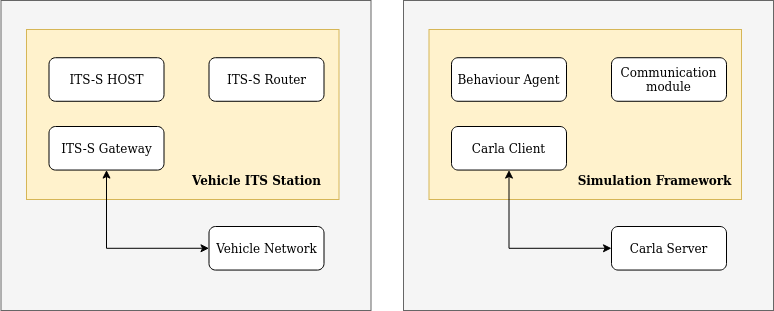
\includegraphics[width=10cm]{Framework/Images/vehicleF.png}.
    \caption{Design of Vehicle ITS Subsystem}
    \label{vehicleF}
\end{figure}

Aforementioned, a vehicle ITS-S installed in vehicles as On Board Unit (OBU). ITS-S host runs the application to control the OBU, it uses IST-S gateway to gather vehicle information for the proprietary vehicular network, and ITS-S router shares it with other Subsystems. Likewise, the framework uses Carla client to collect the ego vehicle information and a communication module shares it with other Carla Client. Additionally, a behaviour Agent controls the behaviour of the ego vehicle. 
The framework provides a waypoint navigation based driving agent to support the ego vehicle mobility as a sub-component of behaviour agent. 


\subsubsection{Design of Roadside Infrastructure}
Roadside infrastructure is standalone devices placed along the road as Road Side Unit (RSU), to control traffic. ITS-S host runs the application to control the RSU. It uses ITS-S router and ITS-S gateway to communicate with other Subsystems and traffic infrastructure (e.g., traffic signal, digital display boards). Similarly, the framework uses the communication module to communicate with the ego vehicle and control module to control the RSU.

\begin{figure}[h!]
    \centering
    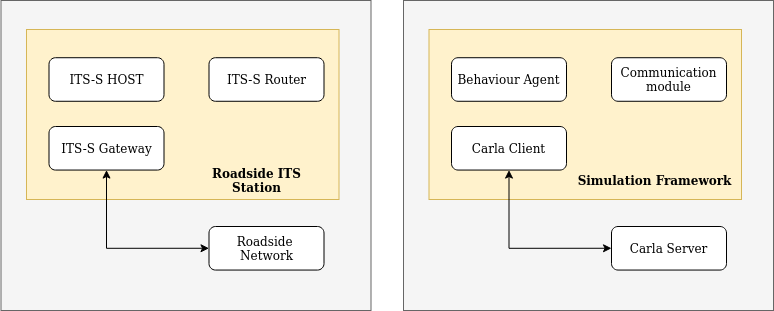
\includegraphics[width=10cm]{Framework/Images/rsuF.png}.
    \caption{Design of Roadside ITS Subsystem}
    \label{rsuF}
\end{figure}


\subsection{Design of Communication Component}
Aforementioned, peer to peer socket communication is performed to share messages between actors. Each actor spawned in the simulation has an attribute called \say{role\_name}, and the framework assigns this attribute with a string combining the Internet Protocol (IP) address and hosts of the actor's socket server (e.g., \say{role\_name} = \say{ip:host}). 

The communication module considers the simulation world created by Carla as a live-map. Before broadcasting a message, it retrieves all the actors \say{role\_name} attribute from the world and sends the message to the actor's socket server.

To broadcast a message only within a filter is created. The role of the filter is to retrieve the \say{role\_name} of the actors within a mentioned range. The filtering is done based on the actor's location in the world.  For instance, consider an RSU that has a communication radius of 200 meters and it needs to broadcast a message. The communication module uses the filter to get the \say{role\_name} of actors within a 200-meter radius of the RSU and broadcasts the message only to those actors. The figure \ref{snip} below is the code snippet of the broadcasting function and \say{isInRange} is the filter function.

\begin{figure}[h!]
    \centering
    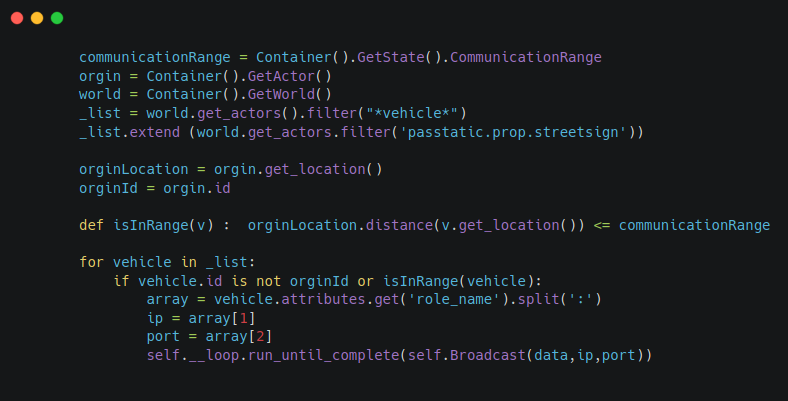
\includegraphics[width=11cm]{Framework/Images/carbon.png}.
    \caption{Broadcast function code snippet}
    \label{snip}
\end{figure}


\subsection{ITS Simulation Performed by the Framework}
 
 The entire design has three main components, the Carla server that takes care of the simulation, the Client that controls the behaviour of actors and the CarlaViz that visualizes the entire thing. 

For instance, consider an RSU is broadcasting a lane closed message and three vehicles moving towards it. The RSU broadcasts the lane change message throughout its life-time. The vehicles spawned at a random location will be moving in its planned path using waypoint navigation until they enter the communication range of RSU. Once a vehicle enters the communication range, it receives the message and changes its path based on the lane id. The sequence diagram in the figure illustrates the message broadcasted by the RSU is only received by the vehicle only when it enters the communication range. Apart from this, the figure shows that the vehicle and RSU behaviour computation is carried out separately by their respective clients, and they coordinate by sending messages.
 
 \begin{figure}[h!]
    \centering
    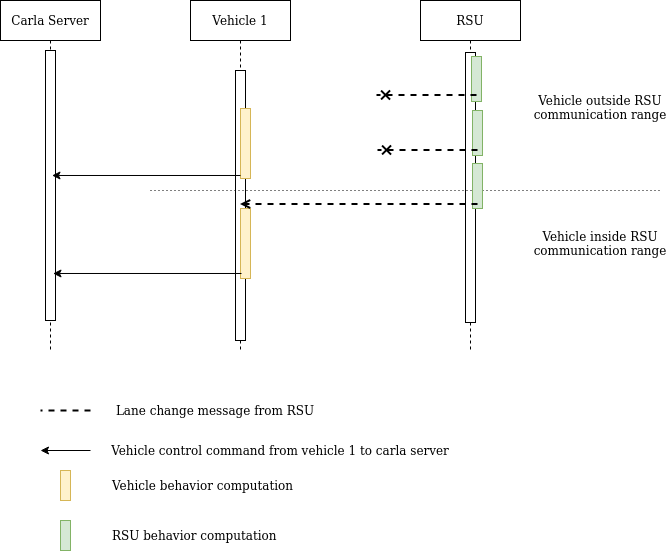
\includegraphics[width=11cm]{Framework/Images/Untitled Diagram(1).png}.
    \caption{Sequence diagram: Simulation Performed by the Framework}
    \label{sequence}
\end{figure}
 
